\section{Mizar}

\begin{minipage}{0.5\textwidth}
\textbf{Name}: Mizar\\
\textbf{Function}: The Antagonist, The Evil Stepmother

\subsection{Internal World}

\textbf{Age \& Gender}: 200, Female \\
\textbf{Values \& Virtues}: Vengeance \\
\textbf{Personality}: Manipulator, Heartless, Egocentric, vindictive \\
\textbf{Interests}: Magic, King of Ingary \\
\textbf{Ethnic Group}: Djinn, Arabic

\subsection{External World}
\textbf{Environment}: The castle of the Kingdom of Strangia. \\
\textbf{Education}: High-educated \\
\textbf{Social \& Cultural Background}: Each people in Strangia respects her because they fear her power. Nobody knows the real reasons why the war is going on. Nobody knows the real story of Mizar \\
\textbf{Look \& Feel}: Her age is 200 but she looks like a 30-35 years old woman. She has pointy ears  \\
\textbf{Job \& Experience}: Court Magician, Queen regent \\

\end{minipage}%
%
\hfill\begin{minipage}{0.4\textwidth}
  \begin{figure}[H]
  
\includegraphics{Images/Characters/mizar}
  %Teniamo questo caption e in futuro mettiamo caption di questo stile quando ci realizzerà qualcosa
  \caption{Sketch of Mizar made by Elena Coperchini}
\end{figure}
\end{minipage}


%% \begin{figure}[H]
%%   
\includegraphics{Images/Characters/mizar}
%%   %Teniamo questo caption e in futuro mettiamo caption di questo stile quando ci realizzerà qualcosa
%%   \caption{Sketch of Mizar made by Elena Coperchini}
%% \end{figure}

%% \textbf{Name}: Mizar\\
%% \textbf{Function}: The Antagonist, The Evil Stepmother

%% \subsection{Internal World}

%% \textbf{Age \& Gender}: 200, Female \\
%% \textbf{Values \& Virtues}: Vengeance \\
%% \textbf{Personality}: Manipulator, Heartless, Egocentric, vindictive \\
%% \textbf{Interests}: Magic, King of Ingary \\
%% \textbf{Ethnic Group}: Djinn, Arabic

%% \subsection{External World}
%% \textbf{Environment}: The castle of the Kingdom of Strangia. \\
%% \textbf{Education}: High-educated \\
%% \textbf{Social \& Cultural Background}: Each people in Strangia respects her because they fear her power. Nobody knows the real reasons why the war is going on. Nobody knows the real story of Mizar \\
%% \textbf{Look \& Feel}: Her age is 200 but she looks like a 30-35 years old woman. She has pointy ears  \\
%% \textbf{Job \& Experience}: Court Magician, Queen regent \\
\\
\textbf{Relatives \& Relation}: Every relation she has is just submission to her.
\begin{itemize}
\item \textbf{Sophie}: She didn’t know Sophie until she tries to defeat her. Since then, Mizar hates her.
\item \textbf{Howl}: She knows him just by reputation but she has never met him until he tries to defeat her. Since then, Mizar hates him. She fears him a bit because rumors say that he is a great wizard.
\item \textbf{Calcifer}: She hates him because he is a friend of Sophie and Howl.
\item \textbf{Belzel}: She doesn’t know him. He is slightly submissive to her and really takes into consideration what she says
\item \textbf{Justin}: He is her stepson. She gets him arrested only because he is a bare  inconvenient with her plans. 
\item \textbf{Suliman}:Mizar has only heard about her, but she still hates her because it’s the new magician of the king of Ingary.
\end{itemize}

\begin{figure}[H]
  \centering
  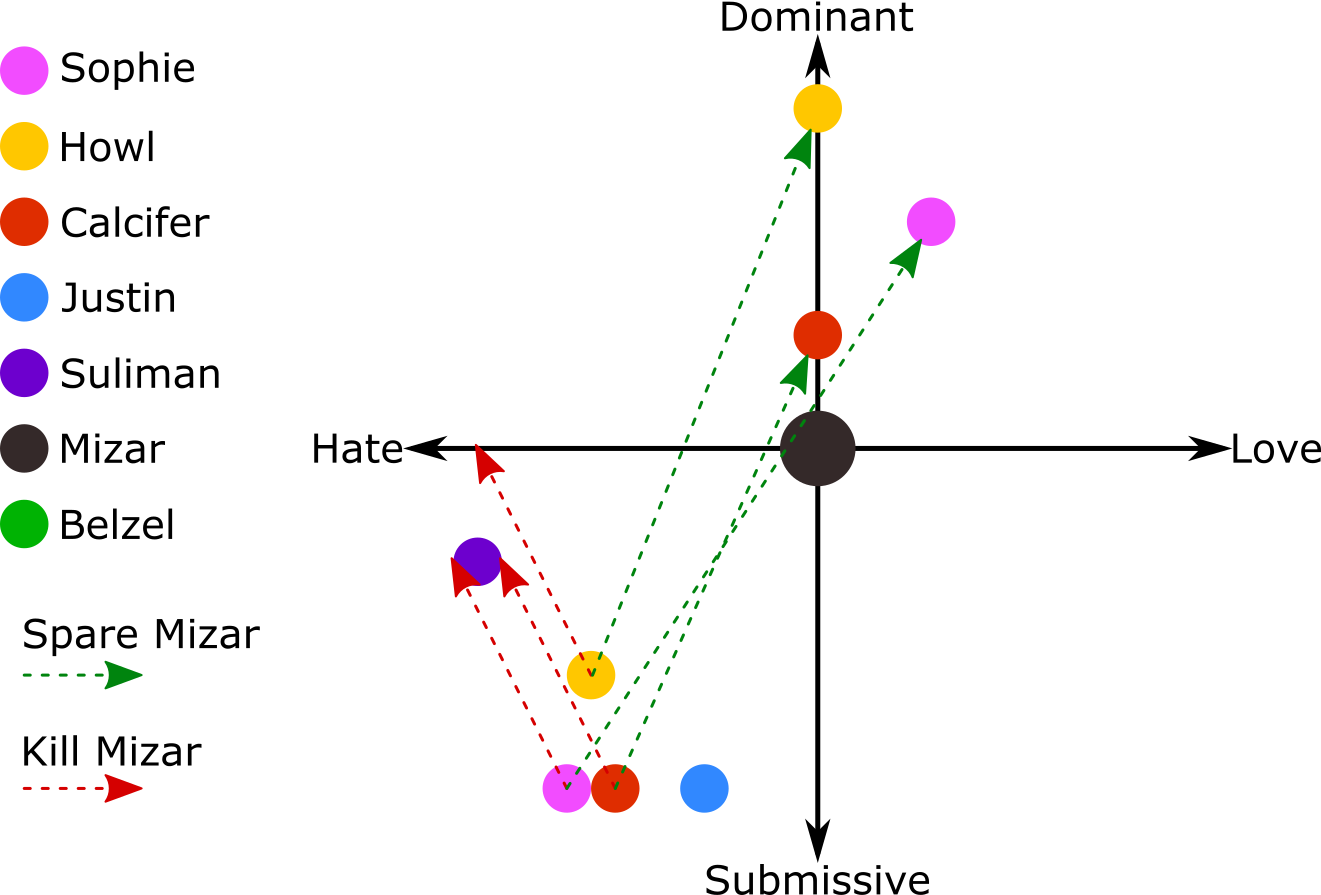
\includegraphics[width=8cm]{Images/Circumplexes/mizarCircumplex}
  \caption{Circumplex of Mizar}
\end{figure}

\begin{figure}[H]
  \centering
  
\includegraphics[width=8cm]{Images/Evolutions/mizarEvolution}
  \caption{Evolutions of Mizar}
\end{figure}

\subsection{Description}
Before being refused, she was the court magician at castle of Ingary. Since she left the castle, she doesn't have any other interest except avenging the humiliation suffered from the king.

She aims to become the most powerful Djinn of the kingdom because she wants to take revenge of the King of Ingary. According to this, she is willing to do anything to make the war go on.

\subsection{Background story}
Her past is unknown.In fact, She is too old for all of the humans beings and nobody knows her story except some of the most recent ones. A long time ago she worked as court magician of the Kingdom of Ingary. She fell in love with the King she declared her love to him, but without the expected results. In fact, the King mocked her and told her he could never love a djinn. She felt humiliated and decided to make him pay for it. She tore out her heart with a spell in order to end her suffering and hid it in a secret place. This act increased his hatred and desire for revenge. Using another spell she charms the king of Strangia and she tricks him in marrying her.
